\documentclass[10pt]{ctexart}
\usepackage{morelull}
\usepackage{enumerate}
\usepackage{bm}
\usepackage{makecell}
\usepackage{xcolor}
\usepackage{graphicx}
\usepackage{subfigure}
\usepackage{framed}%包中有添加文字背景色命令shaded
\colorlet{shadecolor}{MaterialBlue50}
\usepackage{tabularx}
\usepackage{multicol}  
\usepackage{multirow}
\usepackage{indentfirst}
\usepackage{amsmath,amssymb,amsthm,bm,bbding,pifont,dsfont}
\usepackage{mathtools}
\usepackage{tikz}
\newcommand{\abs}[1]{\left| #1 \right|}
\usepackage{caption}
\captionsetup[figure]{labelfont={bf},labelformat={default},labelsep=period,name={图}}
%定义选择题选项
\newcommand{\onech}[4]{
\renewcommand\arraystretch{1.4}
\begin{tabularx}{\linewidth}{XXXX}
\setlength\tabcolsep{0pt}
(A) #1 & (B) #2 & (C) #3 & (D) #4 \\
\end{tabularx}
\unskip \unskip}
\newcommand{\twoch}[4]{
\renewcommand\arraystretch{1.4}
\begin{tabularx}{\linewidth}{XX}
\setlength\tabcolsep{0pt}
(A) #1 & (B) #2 \\
(C) #3 & (D) #4
\end{tabularx}
\unskip \unskip}

%平行四边形
\newcommand*\pxsbx{%
	\mathord{\text{%
			\tikz[baseline]
			\draw (0,.1ex) -- (.8em,.1ex) -- (1em,1.4ex) -- (.2em,1.4ex) -- cycle;}}}

\title{模型研究系列 \quad 截长补短模型}
\author{一粒沙整理\\安徽省霍邱县龙潭中学}
\date{\today}



\begin{document}
\maketitle
\tableofcontents


\section{引入}
截长补短法,是初中几何题中一种添加辅助线的方法,也是把几何题化难为易的一种策略。截长补短的方法适用于求证线段的和差倍分关系。截长,指在长线段中截取一段等于已知线段;补短,指将短线段延长,延长部分等于已知线段。该类题目中常出现等腰三角形、角平分线等关键词句,可以采用截长补短法构造全等三角形来完成证明过程。

\section{截长补短模型}
如图\ding{192},若证明线段$AB$、$CD$、$EF$之间存在$EF=AB+CD$,可以考虑截长补短法。

截长法:如图\ding{193},在$EF$上截取$EG=AB$,再证明$GF=CD$即可。

补短法:如图\ding{194},延长$AB$至$H$点,使$BH=CD$,再证明$AH=EF$即可。

\begin{center}
	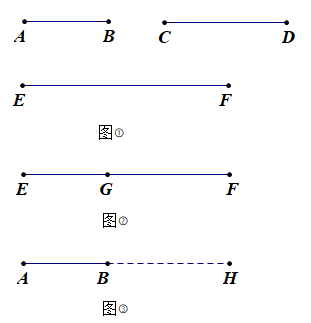
\includegraphics[scale=0.6]{figure/jiechangbuduan01}
\end{center}

\section{例题学习}
\begin{shaded}
	\begin{example}
如图,已知在$\triangle ABC$中,$\angle C=2\angle B$,$AD$平分$\angle BAC$交$BC$于点$D$.

求证:$AB=AC+CD$.
	\end{example}
\end{shaded}

\begin{flushright}
	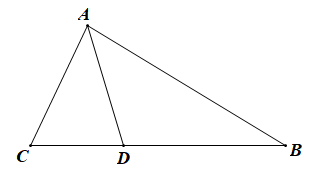
\includegraphics[scale=0.6]{figure/jiechangbuduan02}
\end{flushright}

\begin{shaded}
	\begin{example}
	如图,已知$OD$平分$\angle AOB$,$DC\perp OA$于点$C$,$\angle A=\angle GBD$.
	
	求证:$AO+BO=2CO$.
	\end{example}
\end{shaded}

\begin{flushright}
	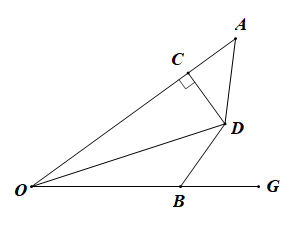
\includegraphics[scale=0.6]{figure/jiechangbuduan03}
\end{flushright}

\begin{shaded}
	\begin{example}
	如图,四边形$ABCD$是正方形,$E,F$分别在$CB,CD$的延长线上,$\angle EAF=135^\circ$.
	
	证明:$BE+DF=EF$.
	\end{example}
\end{shaded}

\begin{flushright}
	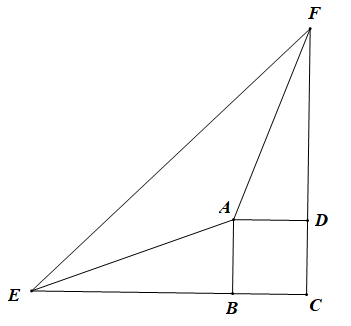
\includegraphics[scale=0.6]{figure/jiechangbuduan11}
\end{flushright}

\section{模型应用}

\begin{shaded}
	1.如图,在$\triangle ABC$中,$\angle BAC=60^\circ$,$AD$是$\angle BAC$的平分线,且$AC=AB+BD$.求$\angle ABC$的度数.
\end{shaded}

\begin{flushright}
	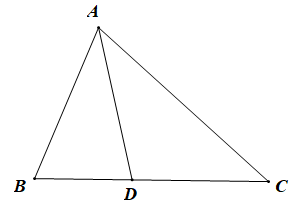
\includegraphics[scale=0.6]{figure/jiechangbuduan04}
\end{flushright}

\begin{shaded}
	2.如图,在$\triangle ABC$中,$\angle ABC=60^\circ$,$AD,CE$分别平分$\angle BAC,\angle ACB$.
	
	求证:$AC=AE+CD$.
\end{shaded}

\begin{flushright}
	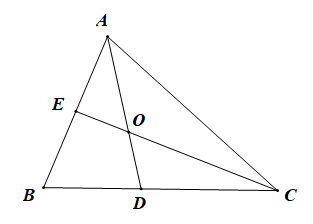
\includegraphics[scale=0.6]{figure/jiechangbuduan05}
\end{flushright}

\begin{shaded}
	3.如图,$\angle ABC+\angle BCD=180^\circ$,$BE,CE$分别平分$\angle ABC,\angle BCD$.
	求证:$AB+CD=BC$.
\end{shaded}

\begin{flushright}
	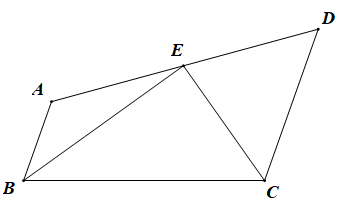
\includegraphics[scale=0.6]{figure/jiechangbuduan06}
\end{flushright}

\begin{shaded}
	4.如图,在$\triangle ABC$中,$\angle ABC=90^\circ$,$AD$平分$\angle BAC$交$BC$于点$D$,$\angle C=30^\circ$,$BE\perp AD$于点$E$.
	
	求证:$AC-AB=2BE$.
\end{shaded}

\begin{flushright}
	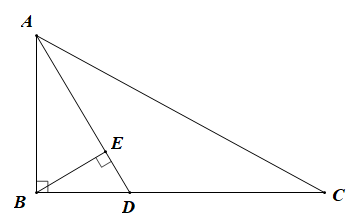
\includegraphics[scale=0.6]{figure/jiechangbuduan07}
\end{flushright}

\begin{shaded}
5.如图,$Rt\triangle ABC$中,$AC=BC$,$AD$平分$\angle BAC$交$BC$于点$D$,$CE\perp AD$交$AD$于$F$点,交$AB$于点$E$.

求证:$AD=2DF+CE$.
\end{shaded}

\begin{flushright}
	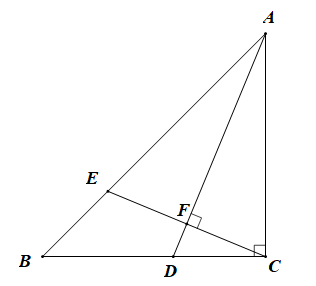
\includegraphics[scale=0.6]{figure/jiechangbuduan08}
\end{flushright}

\begin{shaded}
6.如图,五边形$ABCDE$中,$AB=AC$,$BC+DE=CD$,$\angle B+\angle E=180^\circ$.

求证:$AD$平分$\angle CDE$.
\end{shaded}

\begin{flushright}
	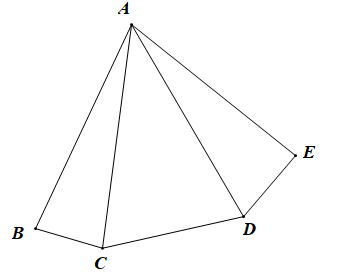
\includegraphics[scale=0.6]{figure/jiechangbuduan09}
\end{flushright}

\begin{shaded}
7.如图,在$\pxsbx ABCD$中,$BE$平分$\angle ABC$交$AD$于点$E$,过点$A$作$AF\perp DC$,交$DC$的延长线于点$F$,分别交$BE,BC$于点$G,H$,且$AB=AF$.

求证:$ED-AG=FC$.
\end{shaded}

\begin{flushright}
	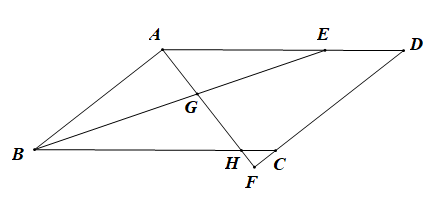
\includegraphics[scale=0.6]{figure/jiechangbuduan10}
\end{flushright}

\begin{shaded}
8.如图,在正方形$ABCD$中,$F$是$CD$的中点,$E$是$BC$边上的一点,且$AF$平分$\angle DAE$.求证:$AE=EC+CD$.
\end{shaded}

\begin{flushright}
	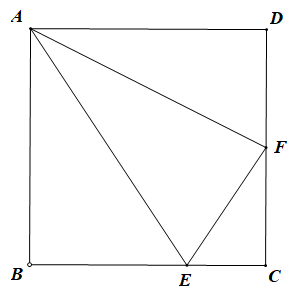
\includegraphics[scale=0.6]{figure/jiechangbuduan12}
\end{flushright}

\begin{shaded}
	9.如图,过平行四边形$ABCD$的顶点$A$的直线$l$(形外),分别过$B,C,D$作直线$l$的垂线,$E,F,G$为垂足。求证:$CF=BE+DG$.
\end{shaded}

\begin{flushright}
	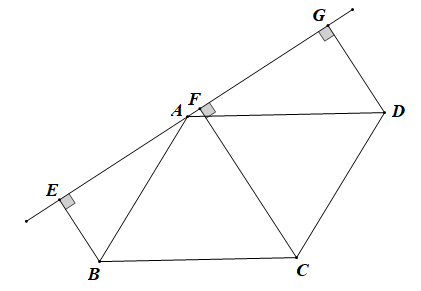
\includegraphics[scale=0.6]{figure/jiechangbuduan13}
\end{flushright}

\begin{shaded}
10.(1)如图1,$\triangle ABC$为等边三角形,点$D$是边$BC$下方一点,$\angle BDC=120^\circ$,探索线段$DA,DB,DC$之间的数量关系.

解题思路:延长$DC$到点$E$,使$CE=BD$,根据$\angle BAC+\angle BDC=120^\circ$,可证$\angle
 ABD=\angle ACE$,易证$\triangle ABD\cong \triangle ACE$,得出$\triangle ADE$是等边三角形,所以$AD=DE$,从而解决问题。根据上述解题思路,三条线段$DA,DB,DC$之间的数量关系是$\underline{\hspace{1.5cm}}$( 直接写出结果);
 
(2)如图2,$Rt\triangle ABC$中,$\angle BAC=90^\circ$,$AB=AC$,点$D$是边$BC$下方一点,$\angle BDC=90^\circ$,探索三线段$DA,DB,DC$之间的等量关系,并证明你的结论。
\end{shaded}

\begin{center}
	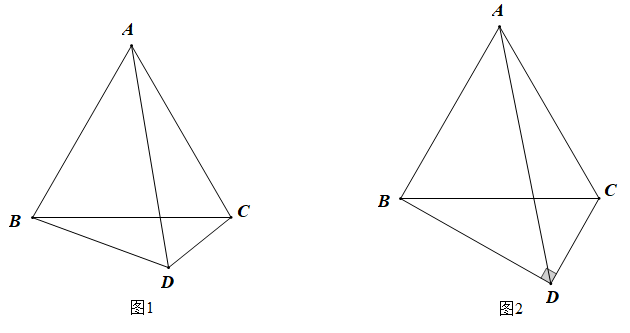
\includegraphics[scale=0.6]{figure/jiechangbuduan14}
\end{center}

\begin{shaded}
	11.如图,在$\triangle ABC$中,$AB=CD-BD,AD\perp BC$.求证:$\angle B=2\angle C$.
\end{shaded}

\begin{flushright}
	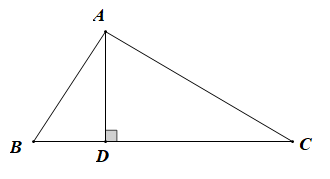
\includegraphics[scale=0.6]{figure/jiechangbuduan15}
\end{flushright}

\begin{shaded}
	12.如图,在$\triangle ABC$中,$AB=AC,∠A=105^\circ$,$BD$平分$\angle ABC$交$AC$于$D$.求证:$BC=AC+CD$.
\end{shaded}

\begin{flushright}
	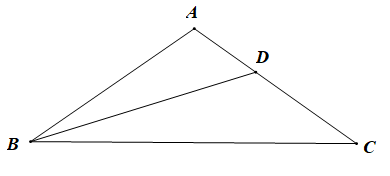
\includegraphics[scale=0.6]{figure/jiechangbuduan16}
\end{flushright}



\end{document}